\chapter{Izvor geometrije}

% \begin{itemize}
%     \item Izraz geometrija izhaja iz grške besede \textit{geometrein}, kjer \textit{geo} pomeni 'zemlja' in \textit{metrein} 'meriti'. Začetki geometrije so torej v zemljemerstvu.
%     \item Grški zgodovinar Herodot (5. stoletje pr. n. št.) pripisuje začetke  geometrije egipčanskim zemljemercem, vendar so imeli pred njimi že Babilonci (2000--1600 pr. n.  št.), Hindujci in Kitajci precej razvito geometrijo. Babilonci so imeli veliko boljše znanje aritmetike in algebre kot Egipčani. Poznali so tudi Pitagorov izrek (veliko pred Pitagoro).
%     \item V začetku je bila geometrija zbirka pravil, do katerih so se dokopali s poskušanjem, analogijami, ugibanjem in občasnimi prebliski intuicije. Tudi približne rešitve so bile večinoma ustrezne za praktične namene.
%     \item Egipčani so včasih uganili pravilno, spet drugič ne; tako so npr. pravilno izračunali volumen pravokotne piramide, za izračun ploščine štirikotnika pa so uporabili kar formulo za ploščino pravokotnika.
% \end{itemize}

    Izraz geometrija izhaja iz grške besede \textit{geometrein}, kjer \textit{geo} pomeni 'zemlja' in \textit{metrein} 'meriti'. Začetki geometrije so torej v zemljemerstvu.

    Grški zgodovinar Herodot (5. stoletje pr. n. št.) pripisuje začetke  geometrije egipčanskim zemljemercem, vendar so imeli pred njimi že Babilonci (2000--1600 pr. n.  št.), Hindujci in Kitajci precej razvito geometrijo. Babilonci so imeli veliko boljše znanje aritmetike in algebre kot Egipčani. Poznali so tudi Pitagorov izrek (veliko pred Pitagoro).

    V začetku je bila geometrija zbirka pravil, do katerih so se dokopali s poskušanjem, analogijami, ugibanjem in občasnimi prebliski intuicije. Tudi približne rešitve so bile večinoma ustrezne za praktične namene.

    Egipčani so včasih uganili pravilno, spet drugič ne; tako so npr. pravilno izračunali volumen pravokotne piramide, za izračun ploščine štirikotnika pa so uporabili kar formulo za ploščino pravokotnika.


\section{Grški prispevek}

% \begin{itemize}
%     \item Grki so, začenši s Talesom iz Mileta (6. stol. pr. n. št.), uvedli logično sklepanje (namesto ugibanja) kot metodo gradnje geometričnega znanja. Bili so prvi, ki so uvedli sistematičen razvoj teorije preko dokazov. Tales je preverjal pravilnost trditev, ki so jih zapustili Egipčani in Babilonci, in tako razvil prvo logično zgrajeno geometrijo.
%     \item Njegovo delo so v naslednjih dveh stoletjih nadaljevali pitagorejci. Sistematične osnove geometrije, ki jih je razvila pitagorejska šola, je okoli leta 400 pr. n. št. zbral v \textit{Elementih} matematik Hippocrates; to delo je bilo kasneje izgubljeno.
%     \item V 4. stoletju pr. n. št. je cvetela Platonova Akademija znanosti in filozofije. Platon je v \textit{Republiki} zapisal: 'Študij matematike razvije in požene v tek mentalni organizem, vreden več kot tisoč oči, saj lahko le skozi tega razumemo resnico.'
%     \item Sokratska metoda dialoga je v bistvu metoda \textit{dokaza s protislovjem}, saj je dokaz nepravilnosti določene izjave to, da le-ta vodi v protislovje.
%     \item Platon je velikokrat citiral dokaz iracionalnosti dolžine diagonale enotskega kvadrata kot ilustracijo dokaza s protislovjem. Bistvo pri tem je, da iracionalnost te dolžine ni mogoče ugotoviti z merjenji, saj ta  vedno vključujejo majhne eksperimentalne napake.
%     \item Za Platona je bil svet idej pomembnejši od materialnega sveta. Menil je, da je napake čutil treba odpraviti s poglobljenim premišljevanjem, ki se ga najbolje naučimo pri študiju matematike.
%     \item Evklid (Eukleidis) iz Aleksandrije je bil naslednik platonske šole. Okoli leta 300 pr. n. št. je v 13. knjigah \textit{Elementov} zbral vso do tedaj razvito geometrijo in teorijo števil. S tem delom je postavil standard aksiomatične metode v matematiki.
%     \item To je bila \textit{čista matematika} v pomenu čiste misli, ki ni potrebovala eksperimentov za preverjanje pravilnosti trditev. Eksperiment ali skico je zamenjal formalen dokaz, tj. izpeljava rezultata s sklepanjem iz aksiomov in preprostejših trditev.
% \end{itemize}

    Grki so, začenši s Talesom iz Mileta (6. stol. pr. n. št.), uvedli logično sklepanje (namesto ugibanja) kot metodo gradnje geometričnega znanja. Bili so prvi, ki so uvedli sistematičen razvoj teorije preko dokazov. Tales je preverjal pravilnost trditev, ki so jih zapustili Egipčani in Babilonci, in tako razvil prvo logično zgrajeno geometrijo.

    Njegovo delo so v naslednjih dveh stoletjih nadaljevali pitagorejci. Sistematične osnove geometrije, ki jih je razvila pitagorejska šola, je okoli leta 400 pr. n. št. zbral v \textit{Elementih} matematik Hippocrates; to delo je bilo kasneje izgubljeno.

    V 4. stoletju pr. n. št. je cvetela Platonova Akademija znanosti in filozofije. Platon je v \textit{Republiki} zapisal: 'Študij matematike razvije in požene v tek mentalni organizem, vreden več kot tisoč oči, saj lahko le skozi tega razumemo resnico.'

    Sokratska metoda dialoga je v bistvu metoda \textit{dokaza s protislovjem}, saj je dokaz nepravilnosti določene izjave to, da le-ta vodi v protislovje.

    Platon je velikokrat citiral dokaz iracionalnosti dolžine diagonale enotskega kvadrata kot ilustracijo dokaza s protislovjem. Bistvo pri tem je, da iracionalnost te dolžine ni mogoče ugotoviti z merjenji, saj ta  vedno vključujejo majhne eksperimentalne napake.

    Za Platona je bil svet idej pomembnejši od materialnega. Menil je, da je napake čutil treba odpraviti s poglobljenim premišljevanjem, ki se ga najbolje naučimo pri študiju matematike.

    Evklid (Eukleidis) iz Aleksandrije je bil naslednik platonske šole. Okoli leta 300 pr. n. št. je v 13. knjigah \textit{Elementov} zbral vso do tedaj razvito geometrijo in teorijo števil. S tem delom je postavil standard aksiomatične metode v matematiki.

    To je bila \textit{čista matematika} v pomenu čiste misli, ki ni potrebovala eksperimentov za preverjanje pravilnosti trditev. Eksperiment ali skico je zamenjal formalen dokaz, tj. izpeljava rezultata s sklepanjem iz aksiomov in preprostejših trditev.


\subsection*{Evklidovi Elementi}

% \begin{multicols}{2}
    \begin{enumerate}[label=\Roman*. knjiga]
        \item Osnove ravninske geometrije
        \item Geometrija pravokotnika
        \item Geometrija kroga
        \item Geometrija pravilnih mnogokotnikov
        \item Geometrija razdalj in razmerij
        \item Geometrija podobnih likov
        \item Osnove aritmetike
        \item Števila in razmerja
        \item Teorija sodih, lihih in perfektnih števil
        \item Neprimerljive dolžine (iracionalna števila)
        \item Osnove geometrije teles
        \item Površine in prostornine teles
        \item Platonska telesa
    \end{enumerate}
% \end{multicols}

\section{Aksiomatična metoda}

% \begin{itemize}
%     \item  Matematiki seveda uporabljamo poskušanje, študij posebnih primerov, navdihnjeno ugibanje in še druge (nestroge) metode za odkrivanje (potencialno pravilnih) trditev.
%     \item Pri (strogem) dokazovanju pravilnosti teh trditev pa nam priskoči na pomoč aksiomatična metoda. Temelj te metode sta naslednji predpostavki:
%         \begin{enumerate}
%             \item Vsi sprejemamo določene trditve, imenovane \textit{aksiomi}, ki ne potrebujejo nobene utemeljitve.
%             \item Vsi sprejemamo \textit{pravila sklepanja}, s pomočjo katerih lahko iz znanih trditev logično izpeljemo nove.
%         \end{enumerate}
%     \item Evklidov najpomembnejši prispevek je, da je izbral majhno število aksiomov, ki so bili sprejemljivi brez utemeljitev, in iz njih izpeljal 465 trditev, med katerimi je prenekatera zapletena in intuitivno ni očitna.
%     \item Evklid je poskušal v \textit{Elementih} definirati vse pojme (prva knjiga vsebuje vse definicije in aksiome). Izkaže se, da to ni mogoče, saj ne moremo definirati vseh pojmov 'nazaj do začetka'. Zato je bolje poleg aksiomov in pravil sklepanja na začetku privzeti tudi nekatere \textit{nedefinirane pojme}.
%     \item Evklid je točko definiral kot \textit{'tisto, ki nima nobenega dela'} in premico kot \textit{'tisto, ki leži na svojih točkah'}. V aksiomatični metodi je torej potrebno privzeti določene pojme. Mi bomo kot nedefinirane vzeli naslednje pojme:
%         \begin{itemize}
%             \item \textit{točka},
%             \item \textit{premica},
%             \item \textit{leži na in leži med},
%             \item \textit{skladen}.
%         \end{itemize}
%         To je Hilbertov nabor nedefiniranih pojmov.
%     \item Ti pojmi dobijo pomen v \textit{modelu}. Evklid je imel ob pisanju definicij v mislih ravninski model (evklidske) geometrije. Osnovne lastnosti pojmov pa bodo zajete v aksiomih.
% \end{itemize}

    Matematiki seveda uporabljamo poskušanje, študij posebnih primerov, navdihnjeno ugibanje in še druge (nestroge) metode za odkrivanje (potencialno pravilnih) trditev.

    Pri (strogem) dokazovanju pravilnosti teh trditev pa nam priskoči na pomoč aksiomatična metoda. Temelj te metode sta naslednji predpostavki:
        \begin{enumerate}
            \item Vsi sprejemamo določene trditve, imenovane \textit{aksiomi}, ki ne potrebujejo nobene utemeljitve.
            \item Vsi sprejemamo \textit{pravila sklepanja}, s pomočjo katerih lahko iz znanih trditev logično izpeljemo nove.
        \end{enumerate}

    Evklidov najpomembnejši prispevek je, da je izbral majhno število aksiomov, ki so bili sprejemljivi brez utemeljitev, in iz njih izpeljal 465 trditev, med katerimi je prenekatera zapletena in intuitivno ni očitna.

    Evklid je poskušal v \textit{Elementih} definirati vse pojme (prva knjiga vsebuje vse definicije in aksiome). Izkaže se, da to ni mogoče, saj ne moremo definirati vseh pojmov 'nazaj do začetka'. Zato je bolje poleg aksiomov in pravil sklepanja na začetku privzeti tudi nekatere \textit{nedefinirane pojme}.

    Evklid je točko definiral kot \textit{'tisto, ki nima nobenega dela'} in premico kot \textit{'tisto, ki leži na svojih točkah'}. V aksiomatični metodi je torej potrebno privzeti določene pojme. Mi bomo kot nedefinirane vzeli naslednje pojme:
        \begin{itemize}
            \item \textit{točka},
            \item \textit{premica},
            \item \textit{leži na in leži med},
            \item \textit{skladen}.
        \end{itemize}
    To je Hilbertov nabor nedefiniranih pojmov.

    Ti pojmi dobijo pomen v \textit{modelu}. Evklid je imel ob pisanju definicij v mislih ravninski model (evklidske) geometrije. Osnovne lastnosti pojmov pa bodo zajete v aksiomih.


\newpage

\section{Evklidovi aksiomi}

\begin{aksiom}[E.1] 
    Za poljubni različni točki $A$ in $B$ obstaja natanko ena premica $p$, ki gre skozi $A$ in $B$.
\end{aksiom}

    \begin{tikzpicture}
        % \clip (0,0) rectangle (14.000000,10.000000);
        {\footnotesize
        
        % Marking point A by circle
        \draw [line width=0.016cm] (2.000000,3.000000) circle (0.040000);%
        \draw (2.030000,2.970000) node [anchor=south east] { $A$ };%
        
        % Marking point B by circle
        \draw [line width=0.016cm] (4.000000,3.500000) circle (0.040000);%
        \draw (4.030000,3.470000) node [anchor=south east] { $B$ };%
        
        % Drawing line p
        \draw [line width=0.016cm] (1.000000,2.750000) -- (1.961194,2.990299);%
        \draw [line width=0.016cm] (2.038806,3.009701) -- (3.961194,3.490299);%
        \draw [line width=0.016cm] (4.038806,3.509701) -- (5.000000,3.750000);%
        }
    \end{tikzpicture}
    
To premico bomo označili z $\overleftrightarrow{AB}$.

\begin{definicija}
    Za različni točki $A$ in $B$ je $\textbf{daljica}$ $AB$ množica točk, ki vsebuje točki $A$ in $B$ ter vse točke na premici $\overleftrightarrow{AB}$, ki ležijo med $A$ in $B$. Točki $A$ in $B$ imenujemo \textbf{krajišči} daljice $AB$.
\end{definicija}

    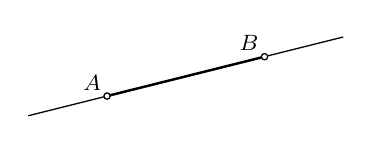
\begin{tikzpicture}
        % \clip (0,0) rectangle (14.000000,10.000000);
        {\footnotesize
        
        % Marking point A by circle
        \draw [line width=0.016cm] (2.000000,3.000000) circle (0.040000);%
        \draw (2.030000,2.970000) node [anchor=south east] { $A$ };%
        
        % Marking point B by circle
        \draw [line width=0.016cm] (4.000000,3.500000) circle (0.040000);%
        \draw (4.030000,3.470000) node [anchor=south east] { $B$ };%
        
        % Drawing line p
        \draw [line width=0.016cm] (1.000000,2.750000) -- (1.961194,2.990299);%
        \draw [line width=0.016cm] (2.038806,3.009701) -- (3.961194,3.490299);%
        \draw [line width=0.016cm] (4.038806,3.509701) -- (5.000000,3.750000);%
        
        % Drawing segment A B
        \draw [line width=0.032cm] (2.038806,3.009701) -- (3.961194,3.490299);%
        }
    \end{tikzpicture}
    

\begin{aksiom}[E.2]
    Za poljubni daljici $AB$ in $CD$ obstaja natanko ena točka $E$, da je $B$ med $A$ in $E$ ter je daljica $CD$ skladna z daljico $BE$.
\end{aksiom}

    \begin{tikzpicture}
        % \clip (0,0) rectangle (14.000000,10.000000);
        {\footnotesize
        
        % Marking point A by circle
        \draw [line width=0.016cm] (2.000000,3.000000) circle (0.040000);%
        \draw (2.030000,2.970000) node [anchor=south east] { $A$ };%
        
        % Marking point B by circle
        \draw [line width=0.016cm] (4.000000,4.500000) circle (0.040000);%
        \draw (4.030000,4.470000) node [anchor=south east] { $B$ };%
        
        % Marking point C by circle
        \draw [line width=0.016cm] (3.000000,1.500000) circle (0.040000);%
        \draw (3.030000,1.470000) node [anchor=south east] { $C$ };%
        
        % Marking point D by circle
        \draw [line width=0.016cm] (5.000000,2.000000) circle (0.040000);%
        \draw (5.030000,1.970000) node [anchor=south east] { $D$ };%
        
        % Drawing line p
        \draw [line width=0.016cm] (6.666667,6.500000) -- (5.679739,5.759804);%
        \draw [line width=0.016cm] (5.618690,5.714017) -- (4.032000,4.524000);%
        \draw [line width=0.016cm] (3.968000,4.476000) -- (2.032000,3.024000);%
        \draw [line width=0.016cm] (1.968000,2.976000) -- (1.000000,2.250000);%
        
        % Drawing line s
        \draw [line width=0.016cm] (1.000000,1.000000) -- (2.961194,1.490299);%
        \draw [line width=0.016cm] (3.038806,1.509701) -- (4.961194,1.990299);%
        \draw [line width=0.016cm] (5.038806,2.009701) -- (7.000000,2.500000);%
        
        % Marking point E by circle
        \draw [line width=0.016cm] (5.656417,5.727307) circle (0.040000);%
        \draw (5.686417,5.697307) node [anchor=south east] { $E$ };%
        
        % Drawing segment B E
        \draw [line width=0.032cm] (4.032139,4.523813) -- (5.624278,5.703493);%
        
        % Drawing segment C D
        \draw [line width=0.032cm] (3.038806,1.509701) -- (4.961194,1.990299);%
        }
        \end{tikzpicture}
        
        
\begin{definicija}
    Za poljubni različni točki $A$ in $B$ imenujemo množico vseh točk $P$, za katere je daljica $AP$ skladna z $AB$, $\textbf{krožnica}$ s $\textbf{središčem}$ $A$. Vsako daljico $AP$ imenujemo $\textbf{polmer}$ krožnice.
\end{definicija}

    \begin{tikzpicture}
        % \clip (0,0) rectangle (14.000000,10.000000);
        {\footnotesize
        
        % Marking point A by circle
        \draw [line width=0.016cm] (4.000000,3.000000) circle (0.040000);%
        \draw (4.030000,2.970000) node [anchor=south east] { $A$ };%
        
        % Marking point B by circle
        \draw [line width=0.016cm] (6.000000,3.500000) circle (0.040000);%
        \draw (5.970000,3.470000) node [anchor=south west] { $B$ };%
        
        % Marking point P
        \draw (4.228878,5.048808) node [anchor=south] { $P$ };%
        
        % Drawing circle p
        \draw [line width=0.016cm] (6.061553,3.000000) arc (0:12:2.061553 and 2.061553) -- (6.009324,3.461102);%
        \draw [line width=0.016cm] (5.989923,3.538710) -- (5.981692,3.568241) arc (16:360:2.061553 and 2.061553) --(6.061553,3.000000) arc (0:0:2.061553 and 2.061553);%
        
        % Drawing segment A B
        \draw [line width=0.016cm] (4.038806,3.009701) -- (5.961194,3.490299);%
        }
    \end{tikzpicture}

\begin{aksiom}[E.3]
    Za poljubni različni točki $A$ in $B$ obstaja krožnica s središčem $A$ in polmerom $AB$.
\end{aksiom}

    Evklid je imel v resnici v mislih konstrukcijo; aksiom torej pravi, da je mogoče krožnico narisati. Naša formulacija v jeziku teorije množic je v bistvu odvečna.

\begin{definicija}
    $\textbf{Poltrak} ~\overrightarrow{AB}$ je naslednja množica točk na premici $\overleftrightarrow{AB}$: vsebuje vse točke na daljici $AB$ in tiste točke $C$ na $\overleftrightarrow{AB}$, za katere je $B$ med $A$ in $C$. Pravimo, da se poltrak $\overrightarrow{AB}$ začne v točki $A$ in da je del premice $\overleftrightarrow{AB}$.
\end{definicija}

    \begin{tikzpicture}
        % \clip (0,0) rectangle (14.000000,10.000000);
        {\footnotesize
        
        % Marking point A by circle
        \draw [line width=0.016cm] (4.000000,3.000000) circle (0.040000);%
        \draw (4.030000,2.970000) node [anchor=south east] { $A$ };%
        
        % Marking point B by circle
        \draw [line width=0.016cm] (6.000000,3.500000) circle (0.040000);%
        \draw (6.030000,3.470000) node [anchor=south east] { $B$ };%
        
        % Marking point C by circle
        \draw [line width=0.016cm] (8.000000,4.000000) circle (0.040000);%
        \draw (8.030000,3.970000) node [anchor=south east] { $C$ };%
        
        % Drawing line p
        \draw [line width=0.016cm] (1.000000,2.250000) -- (3.961194,2.990299);%
        \draw [line width=0.016cm] (4.038806,3.009701) -- (5.961194,3.490299);%
        \draw [line width=0.016cm] (6.038806,3.509701) -- (7.961194,3.990299);%
        \draw [line width=0.016cm] (8.038806,4.009701) -- (9.000000,4.250000);%
        
        % Drawing segment A D
        \draw [line width=0.032cm] (4.038806,3.009701) -- (5.961194,3.490299);%
        \draw [line width=0.032cm] (6.038806,3.509701) -- (7.961194,3.990299);%
        \draw [line width=0.032cm] (8.038806,4.009701) -- (9.000000,4.250000);%
        }
    \end{tikzpicture}
    

\begin{definicija}
    Poltraka $\overrightarrow{AB}$ in $\overrightarrow{AC}$ sta $\textbf{nasprotna}$, če sta različna, se začneta v isti točki $A$ in sta del iste premice $\overleftrightarrow{AB}=\overleftrightarrow{AC}$
\end{definicija}

    \begin{tikzpicture}
        % \clip (0,0) rectangle (14.000000,10.000000);
        {\footnotesize
        
        % Marking point A by circle
        \draw [line width=0.016cm] (6.000000,3.500000) circle (0.040000);%
        \draw (6.030000,3.470000) node [anchor=south east] { $A$ };%
        
        % Marking point B by circle
        \draw [line width=0.016cm] (4.000000,3.000000) circle (0.040000);%
        \draw (4.030000,2.970000) node [anchor=south east] { $B$ };%
        
        % Marking point C by circle
        \draw [line width=0.016cm] (8.000000,4.000000) circle (0.040000);%
        \draw (8.030000,3.970000) node [anchor=south east] { $C$ };%
        
        % Drawing line p
        \draw [line width=0.016cm] (1.500000,2.375000) -- (3.961194,2.990299);%
        \draw [line width=0.016cm] (4.038806,3.009701) -- (5.961194,3.490299);%
        \draw [line width=0.016cm] (6.038806,3.509701) -- (7.961194,3.990299);%
        \draw [line width=0.016cm] (8.038806,4.009701) -- (9.000000,4.250000);%
        
        % Drawing segment A D
        \draw [line width=0.032cm] (6.038806,3.509701) -- (7.961194,3.990299);%
        \draw [line width=0.032cm] (8.038806,4.009701) -- (9.000000,4.250000);%
        }
    \end{tikzpicture}
    

\begin{definicija}
    $\textbf{Kot z vrhom pri}~A$ je točka $A$ skupaj z dvema različnima poltrakoma $\overrightarrow{AB}$ in $\overrightarrow{AC}$, ki nista nasprotna. Poltraka imenujemo $\textbf{stranici}$ kota. Ta kot označimo z $\angle A$ ali $\angle BAC$ ali $\angle CAB$.
\end{definicija}

    \begin{tikzpicture}
        % \clip (0,0) rectangle (14.000000,10.000000);
        {\footnotesize
        
        % Marking point A by circle
        \draw [line width=0.016cm] (2.000000,3.500000) circle (0.040000);%
        \draw (2.030000,3.470000) node [anchor=south east] { $A$ };%
        
        % Marking point B by circle
        \draw [line width=0.016cm] (5.000000,7.000000) circle (0.040000);%
        \draw (5.030000,6.970000) node [anchor=south east] { $B$ };%
        
        % Marking point C by circle
        \draw [line width=0.016cm] (6.000000,4.000000) circle (0.040000);%
        \draw (6.030000,3.970000) node [anchor=south east] { $C$ };%
        
        % Drawing line p
        \draw [line width=0.016cm] (5.857143,8.000000) -- (5.026032,7.030370);%
        \draw [line width=0.016cm] (4.973968,6.969630) -- (2.026032,3.530370);%
        \draw [line width=0.016cm] (1.973968,3.469630) -- (1.000000,2.333333);%
        
        % Drawing line r
        \draw [line width=0.016cm] (1.000000,3.375000) -- (1.960309,3.495039);%
        \draw [line width=0.016cm] (2.039691,3.504961) -- (5.960309,3.995039);%
        \draw [line width=0.016cm] (6.039691,4.004961) -- (9.000000,4.375000);%
        
        % Drawing segment A D
        \draw [line width=0.032cm] (5.857143,8.000000) -- (5.026032,7.030370);%
        \draw [line width=0.032cm] (4.973968,6.969630) -- (2.026032,3.530370);%
        
        % Drawing segment A E
        \draw [line width=0.032cm] (2.039691,3.504961) -- (5.960309,3.995039);%
        \draw [line width=0.032cm] (6.039691,4.004961) -- (9.000000,4.375000);%
        }
    \end{tikzpicture}
    

\begin{definicija}
    Če imata kota $\angle BAD$ in $\angle CAD$ skupno stranico $\overrightarrow{AD}$ in sta drugi stranici $\overrightarrow{AB}$ in $\overrightarrow{AC}$ nasprotna poltraka, imenujemo kota $\textbf{suplementarna}$.
\end{definicija}

    \begin{tikzpicture}
        % \clip (0,0) rectangle (14.000000,10.000000);
        {\footnotesize
        
        % Marking point A by circle
        \draw [line width=0.016cm] (4.000000,4.000000) circle (0.040000);%
        \draw (4.030000,3.970000) node [anchor=south east] { $A$ };%
        
        % Marking point B by circle
        \draw [line width=0.016cm] (7.000000,4.000000) circle (0.040000);%
        \draw (7.030000,3.970000) node [anchor=south east] { $B$ };%
        
        % Marking point C by circle
        \draw [line width=0.016cm] (2.000000,4.000000) circle (0.040000);%
        \draw (2.030000,3.970000) node [anchor=south east] { $C$ };%
        
        % Marking point D by circle
        \draw [line width=0.016cm] (5.000000,6.000000) circle (0.040000);%
        \draw (5.030000,5.970000) node [anchor=south east] { $D$ };%
        
        % Drawing line p
        \draw [line width=0.016cm] (1.000000,4.000000) -- (1.960000,4.000000);%
        \draw [line width=0.016cm] (2.040000,4.000000) -- (3.960000,4.000000);%
        \draw [line width=0.016cm] (4.040000,4.000000) -- (6.960000,4.000000);%
        \draw [line width=0.016cm] (7.040000,4.000000) -- (8.500000,4.000000);%
        
        % Drawing line r
        \draw [line width=0.016cm] (1.000000,4.000000) -- (1.960000,4.000000);%
        \draw [line width=0.016cm] (2.040000,4.000000) -- (3.960000,4.000000);%
        \draw [line width=0.016cm] (4.040000,4.000000) -- (6.960000,4.000000);%
        \draw [line width=0.016cm] (7.040000,4.000000) -- (8.500000,4.000000);%
        
        % Drawing line s
        \draw [line width=0.016cm] (3.750000,3.500000) -- (3.982111,3.964223);%
        \draw [line width=0.016cm] (4.017889,4.035777) -- (4.982111,5.964223);%
        \draw [line width=0.016cm] (5.017889,6.035777) -- (5.500000,7.000000);%
        }
    \end{tikzpicture}
    

\begin{definicija}
    Kot $\angle BAD$ je $\textbf{pravi kot}$, če ima skladen suplementaren kot.
\end{definicija}

    \begin{tikzpicture}
        % \clip (0,0) rectangle (14.000000,10.000000);
        {\footnotesize
        
        % Marking point A by circle
        \draw [line width=0.016cm] (4.000000,4.000000) circle (0.040000);%
        \draw (4.030000,3.970000) node [anchor=south east] { $A$ };%
        
        % Marking point B by circle
        \draw [line width=0.016cm] (7.000000,4.000000) circle (0.040000);%
        \draw (7.030000,3.970000) node [anchor=south east] { $B$ };%
        
        % Marking point C by circle
        \draw [line width=0.016cm] (2.000000,4.000000) circle (0.040000);%
        \draw (2.030000,3.970000) node [anchor=south east] { $C$ };%
        
        % Marking point D by circle
        \draw [line width=0.016cm] (4.000000,6.000000) circle (0.040000);%
        \draw (4.030000,5.970000) node [anchor=south east] { $D$ };%
        
        % Drawing line p
        \draw [line width=0.016cm] (1.000000,4.000000) -- (1.960000,4.000000);%
        \draw [line width=0.016cm] (2.040000,4.000000) -- (3.960000,4.000000);%
        \draw [line width=0.016cm] (4.040000,4.000000) -- (6.960000,4.000000);%
        \draw [line width=0.016cm] (7.040000,4.000000) -- (8.500000,4.000000);%
        
        % Drawing line r
        \draw [line width=0.016cm] (1.000000,4.000000) -- (1.960000,4.000000);%
        \draw [line width=0.016cm] (2.040000,4.000000) -- (3.960000,4.000000);%
        \draw [line width=0.016cm] (4.040000,4.000000) -- (6.960000,4.000000);%
        \draw [line width=0.016cm] (7.040000,4.000000) -- (8.500000,4.000000);%
        
        % Drawing line s
        \draw [line width=0.016cm] (4.000000,3.500000) -- (4.000000,3.960000);%
        \draw [line width=0.016cm] (4.000000,4.040000) -- (4.000000,5.960000);%
        \draw [line width=0.016cm] (4.000000,6.040000) -- (4.000000,7.000000);%
        }
    \end{tikzpicture}
    

\begin{aksiom}[E.4]
    Vsi pravi koti so skladni.
\end{aksiom}


\begin{definicija}
    Premici $p$ in $q$ sta $\textbf{vzporedni}$, če se ne sekata (tj. nimata skupnih točk). Oznaka $p\parallel q$.
\end{definicija}

\begin{aksiom}[E.5]
    Za vsako premico $p$ in vsako točko $A$, ki ne leži na $p$, obstaja natanko ena premica $q$ skozi $A$, ki je vzporedna $p$.
\end{aksiom}

    \begin{tikzpicture}
        % \clip (0,0) rectangle (14.000000,10.000000);
        {\footnotesize
        
        % Marking point A by circle
        \draw [line width=0.016cm] (5.000000,6.000000) circle (0.040000);%
        \draw (5.030000,5.970000) node [anchor=south east] { $A$ };%
        
        % Marking point p
        \draw (7.000000,4.500000) node [anchor=south east] { $p$ };%
        
        % Marking point q
        \draw (6.702703,6.283784) node [anchor=south east] { $q$ };%
        
        % Drawing line r
        \draw [line width=0.016cm] (1.000000,3.500000) -- (8.500000,4.750000);%
        
        % Drawing line s
        \draw [line width=0.016cm] (1.000000,5.333333) -- (4.960544,5.993424);%
        \draw [line width=0.016cm] (5.039456,6.006576) -- (8.500000,6.583333);%
        }
    \end{tikzpicture}
    